\chapter{Introduction}
\makeheading{Week 1}
\section{Notation and Nomenclature}
\begin{Example}{Experiment 1 --- List View vs. Tile View}{nike_ex}
    Suppose that \href{https://www.nike.com/ca/}{Nike}, the athletic apparel company,
    is experimenting with their mobile shopping interface, and they are interested in determining
    whether changing the user interface from \emph{list view}
    to \emph{tile view} will increase the proportion
    of customers that proceed to checkout.
\end{Example}
\begin{Example}{Experiment 2 --- Ad Themes}{nixon_ex}
    Suppose that \href{https://www.nixon.com/ca/en}{Nixon},
    the watch and accessories brand, is experimenting
    with four different video ads that are to be shown on Instagram.
    The first has a surfing theme, the second has a rock climbing theme, the third
    has a camping theme, and the fourth has an urban professional theme.
    Interest lies in determining which of the four themes, on average,
    is watched the longest.
\end{Example}
\begin{Definition}{Metric of interest}{}
    The \textbf{metric of interest} (MOI) is the statistic we wish
    the experiment investigates.
\end{Definition}
\begin{Remark}{}{}
    Typically, we want to optimize for the metric of interest; that is,
    we would like to either maximize or minimize it.
\end{Remark}
\begin{Example}{Metric of Interest}{}
    \begin{itemize}
        \item Key performance indicators (KPIs): a statistic that
              quantifies something about a business.
              \begin{itemize}
                  \item Click-through rates (CTRs).
                  \item Bounce rate.
                  \item Average time on page.
                  \item $ 95^{\text{th}} $ percentile page load time.
              \end{itemize}
        \item \emph{\hyperref[ex:nike_ex]{Nike Example}}: checkout rate (COR).
        \item \emph{\hyperref[ex:nixon_ex]{Nixon Example}}: average viewing duration (AVD).
    \end{itemize}
\end{Example}
\begin{Definition}{Response variable}{}
    The \textbf{response variable}, denoted $ y $, is the variable of primary interest.
\end{Definition}
\begin{Remark}{}{}
    The response variable is what needs to be measured in order for the MOI to be calculated.
\end{Remark}
\begin{Example}{Response Variable}{}
    \begin{itemize}
        \item \emph{\hyperref[ex:nike_ex]{Nike Example}}: binary indicator indicating
              whether a customer checked out.
        \item \emph{\hyperref[ex:nixon_ex]{Nixon Example}}: the continuous measurement
              of viewing duration for each user.
    \end{itemize}
\end{Example}
\begin{Definition}{Factor}{}
    The \textbf{factor}, denoted $ x $, is the variable(s) of secondary interest.

    \vspace{2mm}

    Also known as: \textbf{covariates}, \textbf{explanatory variates}, \textbf{predictors},
    \textbf{features}, \textbf{independent variables}.
\end{Definition}
\begin{Remark}{}{}
    We usually think the factors influence the response (dependent) variable.
\end{Remark}
\begin{Example}{Factor}{}
    \begin{itemize}
        \item \emph{\hyperref[ex:nike_ex]{Nike Example}}: the factor is the \emph{visual layout}.
        \item \emph{\hyperref[ex:nixon_ex]{Nixon Example}}: the factor is the \emph{ad theme}.
    \end{itemize}
\end{Example}
\begin{Definition}{Experimental conditions}{}
    The \textbf{experimental conditions} are the unique combinations of levels of one or more
    factors.

    \vspace{2mm}

    Also known as: \textbf{treatments}, \textbf{variants}, \textbf{buckets}.
\end{Definition}
\begin{Definition}{Levels}{}
    The \textbf{levels} are the values that a factor takes on in an experiment.
\end{Definition}
\begin{Example}{Levels}{}
    \begin{itemize}
        \item \emph{\hyperref[ex:nike_ex]{Nike Example}}: $ \Set*{\text{tile view}, \text{list view}} $.
        \item \emph{\hyperref[ex:nixon_ex]{Nixon Example}}: $ \Set*{\text{surfing}, \text{rock climbing}, \text{camping}, \text{business}} $.
    \end{itemize}
\end{Example}
\begin{Definition}{Experimental units}{}
    The \textbf{experimental units} are what is assigned to the experimental conditions,
    and on which we measure the response variable.
\end{Definition}
\begin{Example}{Experimental Units}{}
    \begin{itemize}
        \item \emph{\hyperref[ex:nike_ex]{Nike Example}}: Nike mobile customers.
        \item \emph{\hyperref[ex:nixon_ex]{Nixon Example}}: Instagram users.
    \end{itemize}
\end{Example}
\begin{Remark}{}{}
    Often, in online experiments, the unit is a user/customer (i.e., person), but it does
    not have to be.
    \begin{Example}{}{}
        Uber matching algorithm experiment.
    \end{Example}
\end{Remark}
\section{Experiments versus Observational Studies}
\begin{Definition}{Experiment}{}
    An \textbf{experiment} is a collection of conditions defined by
    \emph{purposeful changes} to one or more factors. Here, we intervene in the data collection.
\end{Definition}
\begin{itemize}
    \item The goal is to identify and quantify the differences in response variable values
          across conditions.
    \item In determining whether a factor significantly influences a response,
          like whether a video ad's theme significantly influences its AVD, it is
          necessary to understand how experimental units' response when exposed to each
          of the corresponding conditions.
    \item However, it would be nice if we could observe how the \emph{same} units behave in
          each of the experimental conditions, but we can't. We only observe their response in a
          single condition.
    \item \textbf{Counterfactual}: the hypothetical and unobservable value of a unit's response
          in a condition to which they were not assigned. We may think of this
          as an ``alternate reality.''
          \begin{Example}{}{}
              \emph{\hyperref[ex:nixon_ex]{Nixon Example}}: the ``camping'' response
              variable for units assigned to the ``surfing'' condition.
          \end{Example}
    \item Because counterfactual outcomes cannot be observed, we require a \textbf{proxy}.
          Instead, we randomly assign \emph{different units} to \emph{different experimental
              conditions},
          and we compare their responses.
    \item Ideally, the only difference between the units in each condition is the fact that
          they are in different conditions.
          \begin{itemize}
              \item We want the units to be as homogenous as possible, this will help facilitate
                    \textbf{causal inference} (establishing causal connections between variables).
              \item This is typically guaranteed by \emph{randomization}.
          \end{itemize}
    \item The key here is that we purposefully control the factors to
          observe the resulting effect on the response. This facilitates causal conclusions.
    \item In an \textbf{observational study}, on the other hand, there is no measure of control
          in the data collection process. Instead, we collect the data passively and
          the relationship between the response and factor(s) is observed organically.
    \item This hinders our ability to establish causal connections between the factor(s)
          and the response variables. However, sometimes we have no choice.
          \begin{Example}{Unethical Experiments}{}
              \begin{itemize}
                  \item \emph{Unethical Experiment 1}: In evaluating whether smoking lung cancer,
                        it would be unethical to have a `\emph{smoking}' condition in which we force the
                        subjects to smoke.
                  \item \emph{Unethical Experiment 2}: In dynamic pricing experiments, it would be unethical
                        to show different users different prices for the same products. For example, surge pricing
                        in Uber/Lyft.
                  \item \emph{Unethical Experiment 3}: In social contagion experiments, it would be unethical
                        to show some network users consistently negative content and others consistently positive content.
                        \href{https://slate.com/technology/2014/06/facebook-unethical-experiment-it-made-news-feeds-happier-or-sadder-to-manipulate-peoples-emotions.html}{But Facebook did this anyway.}
                  \item \emph{Unethical Experiment 4}: Mozilla conducted an investigation in which
                        the company was interested in determining whether Firefox users that installed an ad blocker
                        were more engaged with the browser. However, it would have been unethical to force users to install
                        an ad blocker, and so they were forced to perform an observational study with \emph{propensity score matching}
                        instead.
              \end{itemize}
          \end{Example}
\end{itemize}
\begin{table}[!htbp]
    \centering
    \begin{NiceTabular}{|>{\raggedright\arraybackslash}m{33mm}|m{50mm}|m{50mm}|}
        \toprule
        & \multicolumn{1}{c}{\emph{Advantages}}                            & \multicolumn{1}{c}{\emph{Disadvantages}}                             \\
        \midrule
        \emph{Experiment}          & Causal inference is clean.                     & Experiments might be unethical, risky, or costly. \\
        \emph{Observational Study} & No additional cost, risk, or ethical concerns. & Causal inference is muddy.\\
        \bottomrule
    \end{NiceTabular}
\end{table}
\section{QPDAC: A Strategy for Answering Questions with Data}
\begin{figure}[!htbp]
    \centering
    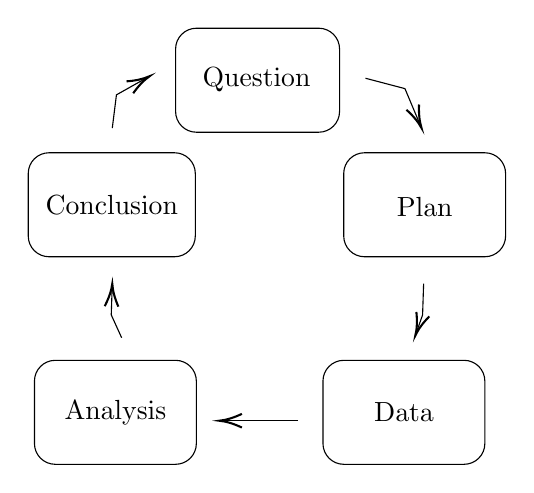
\begin{tikzpicture}[x=0.75pt,y=0.75pt,yscale=-1,xscale=1]
        %Rounded Rect [id:dp4108411703079956] 
        \draw   (90.8,21.02) .. controls (90.8,15.49) and (95.29,11) .. (100.82,11) -- (159.78,11) .. controls (165.31,11) and (169.8,15.49) .. (169.8,21.02) -- (169.8,51.08) .. controls (169.8,56.61) and (165.31,61.1) .. (159.78,61.1) -- (100.82,61.1) .. controls (95.29,61.1) and (90.8,56.61) .. (90.8,51.08) -- cycle ;
        %Straight Lines [id:da741997150285443] 
        \draw    (182.3,35.1) -- (201.3,40.1) -- (208.52,57.26) ;
        \draw [shift={(209.3,59.1)}, rotate = 247.17000000000002] [color={rgb, 255:red, 0; green, 0; blue, 0 }  ][line width=0.75]    (10.93,-3.29) .. controls (6.95,-1.4) and (3.31,-0.3) .. (0,0) .. controls (3.31,0.3) and (6.95,1.4) .. (10.93,3.29)   ;
        %Rounded Rect [id:dp46698747125928275] 
        \draw   (171.8,81.02) .. controls (171.8,75.49) and (176.29,71) .. (181.82,71) -- (239.78,71) .. controls (245.31,71) and (249.8,75.49) .. (249.8,81.02) -- (249.8,111.08) .. controls (249.8,116.61) and (245.31,121.1) .. (239.78,121.1) -- (181.82,121.1) .. controls (176.29,121.1) and (171.8,116.61) .. (171.8,111.08) -- cycle ;
        %Rounded Rect [id:dp7263344152879622] 
        \draw   (161.8,181.02) .. controls (161.8,175.49) and (166.29,171) .. (171.82,171) -- (229.78,171) .. controls (235.31,171) and (239.8,175.49) .. (239.8,181.02) -- (239.8,211.08) .. controls (239.8,216.61) and (235.31,221.1) .. (229.78,221.1) -- (171.82,221.1) .. controls (166.29,221.1) and (161.8,216.61) .. (161.8,211.08) -- cycle ;
        %Straight Lines [id:da2954560098777831] 
        \draw    (149.8,200.1) -- (113.8,200.1) ;
        \draw [shift={(111.8,200.1)}, rotate = 360] [color={rgb, 255:red, 0; green, 0; blue, 0 }  ][line width=0.75]    (10.93,-3.29) .. controls (6.95,-1.4) and (3.31,-0.3) .. (0,0) .. controls (3.31,0.3) and (6.95,1.4) .. (10.93,3.29)   ;
        %Rounded Rect [id:dp9388941577264861] 
        \draw   (22.8,181.02) .. controls (22.8,175.49) and (27.29,171) .. (32.82,171) -- (90.78,171) .. controls (96.31,171) and (100.8,175.49) .. (100.8,181.02) -- (100.8,211.08) .. controls (100.8,216.61) and (96.31,221.1) .. (90.78,221.1) -- (32.82,221.1) .. controls (27.29,221.1) and (22.8,216.61) .. (22.8,211.08) -- cycle ;
        %Straight Lines [id:da06214244678902836] 
        \draw    (60.23,136.1) -- (59.8,149.1) -- (64.8,160.1) ;
        \draw [shift={(60.3,134.1)}, rotate = 91.91] [color={rgb, 255:red, 0; green, 0; blue, 0 }  ][line width=0.75]    (10.93,-3.29) .. controls (6.95,-1.4) and (3.31,-0.3) .. (0,0) .. controls (3.31,0.3) and (6.95,1.4) .. (10.93,3.29)   ;
        %Rounded Rect [id:dp17859829449373688] 
        \draw   (19.8,81.02) .. controls (19.8,75.49) and (24.29,71) .. (29.82,71) -- (90.28,71) .. controls (95.81,71) and (100.3,75.49) .. (100.3,81.02) -- (100.3,111.08) .. controls (100.3,116.61) and (95.81,121.1) .. (90.28,121.1) -- (29.82,121.1) .. controls (24.29,121.1) and (19.8,116.61) .. (19.8,111.08) -- cycle ;
        %Straight Lines [id:da4605450389949781] 
        \draw    (76.56,35.08) -- (62.3,43.1) -- (60.3,59.1) ;
        \draw [shift={(78.3,34.1)}, rotate = 150.64] [color={rgb, 255:red, 0; green, 0; blue, 0 }  ][line width=0.75]    (10.93,-3.29) .. controls (6.95,-1.4) and (3.31,-0.3) .. (0,0) .. controls (3.31,0.3) and (6.95,1.4) .. (10.93,3.29)   ;
        %Straight Lines [id:da28852075027489266] 
        \draw    (210.3,134.1) -- (209.8,149.1) -- (206.96,157.21) ;
        \draw [shift={(206.3,159.1)}, rotate = 289.29] [color={rgb, 255:red, 0; green, 0; blue, 0 }  ][line width=0.75]    (10.93,-3.29) .. controls (6.95,-1.4) and (3.31,-0.3) .. (0,0) .. controls (3.31,0.3) and (6.95,1.4) .. (10.93,3.29)   ;

        % Text Node
        \draw (129.8,36.05) node   [align=left] {Question};
        % Text Node
        \draw (210.8,97.05) node   [align=left] {Plan};
        % Text Node
        \draw (200.8,196.05) node   [align=left] {Data};
        % Text Node
        \draw (61.8,196.05) node   [align=left] {Analysis};
        % Text Node
        \draw (60.05,96.05) node   [align=left] {Conclusion};
    \end{tikzpicture}
    \caption{QPDAC Cycle}
\end{figure}
\begin{framed}
    \textbf{Question}: Develop a clear statement of the question that needs to be answered.
    \begin{itemize}
        \item It is important that this is clear and concise and widely communicated,
              so all stakeholders are on the same page.
        \item The question should be quantifiable/measurable and typically stated
              in terms of the metric of interest.
    \end{itemize}
    \begin{Example}{}{}
        \begin{itemize}
            \item \emph{\hyperref[ex:nike_ex]{Nike Example}}: ``which visual layout, tile view
                  or list view, corresponds to the highest checkout rate?''
            \item \emph{\hyperref[ex:nixon_ex]{Nixon Example}}:
                  ``which ad theme, camping, surfing, rock climbing, business, corresponds to
                  the highest average viewing duration?''
        \end{itemize}
    \end{Example}
\end{framed}
\begin{framed}
    \textbf{Plan}: In this stage, we design the experiment, and all pre-experimental questions
    should be answered.
    \begin{itemize}
        \item Choose the response variable. This should be dictated by the \textbf{Question} and the metric
              of interest.
        \item Choose the factor(s): brainstorm all factors that might influence the response and make
              decisions about whether and how they will be controlled in the experiment.
              \begin{enumerate}[i]
                  \item \textbf{Design factors}: factors that we will manipulate in the experiment.
                        The factors we've discussed in the Nike and Nixon examples are design factors.
                  \item \textbf{Nuisance factors}: factors that we expect to influence
                        the response, but whose effect we do not care to quantify. Instead, we try to eliminate
                        their effects with \emph{blocking}.
                  \item \textbf{Allowed-to-vary factors}: factors that we \emph{cannot} control and factors that
                        we are unaware of in an experiment.
                        \begin{itemize}
                            \item \emph{\hyperref[ex:nixon_ex]{Nixon Example}}:
                                  users' age, gender, nationality.
                        \end{itemize}
              \end{enumerate}
        \item Choose the experimental units. These are what we measure the response variable on.
        \item Choose the sample size and sampling mechanism.
              \begin{itemize}
                  \item Sample size: how many units per experimental condition?
                  \item Sampling mechanism: how are they selected?
              \end{itemize}
    \end{itemize}
\end{framed}
\begin{framed}
    \textbf{Data}: In this stage, we collect the data according to the \textbf{Plan}.
    It is extremely important that we do this step correctly; the suitability and effectiveness
    of the analysis relies on the correctness of the data. Computer scientists often
    use the phrase
    ``garbage in, garbage out'' to describe the phenomenon whereby poor
    quality input will always provide faulty output.
    \begin{itemize}
        \item A/A Test: we assign units to one of two \emph{identical} conditions.
              \begin{itemize}
                  \item We do this to ensure the assignment of units to conditions is truly random.
                  \item Two groups should be indistinguishable in terms of response distribution
                        and other demographics.
                  \item If things aren't indistinguishable, there is a problem.
                  \item \emph{Sample Ratio Mismatch Test}: If the ratio of users
                        (or any randomization unit) between the variants is not close
                        to the designed ratio, the experiment suffers from a Sample Ratio Mismatch
                        (SRM).
                        \begin{itemize}
                            \item Hypothesis test can be used to determine whether the proportion
                                  of units in each condition match what would have been expected under
                                  random assignment.
                        \end{itemize}
              \end{itemize}
    \end{itemize}
\end{framed}
\begin{framed}
    \textbf{Analysis}: In this stage, we statistically analyze \textbf{Data}
    to provide an objective answer to the \textbf{Question}.
    \begin{itemize}
        \item This is typically achieved by way of estimating parameters, fitting models,
              and carrying out statistical hypothesis tests. This is where we spend most of
              our time in the course.
        \item If the experiment was well-designed, and we collected the data correctly, this
              step should be straight-forward.
    \end{itemize}
\end{framed}
\begin{framed}
    \textbf{Conclusion}: In this stage, we consider the results of the \textbf{Analysis},
    and one must draw conclusions about what has been learned.
    \begin{itemize}
        \item We clearly communicate these conclusions to all parties involved
              in --- or impacted by --- the experiment.
        \item Communicating ``wins'' and ``loses'' will help to foster the culture
              of experimentation.
    \end{itemize}
\end{framed}
\section{Fundamental Principles of Experimental Design}
\begin{Definition}{Randomization}{}
    \textbf{Randomization} refers both to the manner in which we select experimental units
    for \emph{inclusion} in the experiment and the manner in which we \emph{assign} them
    to \emph{experimental conditions}.
\end{Definition}
\begin{Remark}{}{}
    Typically, we don't include the entire target/study population.
\end{Remark}
Thus, we have two levels of randomization:
\begin{itemize}
    \item The first level of randomization exists to ensure the sample of units included in
          the experiment is \emph{representative of those that were not}.
          \begin{itemize}
              \item Allows us to generalize conclusions beyond just the experimental units to units
                    in the population not in the experiment.
          \end{itemize}
    \item The second level of randomization exists to \emph{balance} the effects of \emph{extraneous variables}
          not under study (i.e., the allowed-to-vary factors).
          \begin{itemize}
              \item Balancing the effects of allowed-to-vary factors makes our conditions homogenous
                    and thus best mimics the counterfactual, thereby making causal inference easy.
          \end{itemize}
\end{itemize}
\begin{Definition}{Replication}{}
    \textbf{Replication} refers to the existence of multiple response observations
    within each experimental condition and thus corresponds to the situation in which
    we assign more than one unit to each condition.
\end{Definition}
\begin{itemize}
    \item Assigning multiple units to each condition provides \emph{assurance} that the
          observed results are genuine, and \emph{not just due to chance}.
    \item For instance, consider the \emph{\hyperref[ex:nike_ex]{Nike experiment}}
          introduced previously. Suppose the CORs in the \emph{list view} and
          \emph{tile view} conditions were 0.5 and 1 respectively. This conclusion would be
          a lot more convincing if each condition had $ n=1000 $ units as opposed to $ n=2 $,
          where $ n $ is the sample size in \emph{each} condition.
    \item How much replication do we need?
          \begin{itemize}
              \item How big a sample size do we need?
              \item Power analysis + sample size calculations will help answer this.
          \end{itemize}
\end{itemize}
\begin{Definition}{Blocking}{}
    \textbf{Blocking} is the mechanism that we control the nuisance factors.
\end{Definition}
\begin{itemize}
    \item To \emph{eliminate} the influence of nuisance factors, we hold them fixed during
          the experiment.
    \item Thus, we run the experiment \emph{at fixed levels of the nuisance factors}, i.e.,
          within \textbf{blocks}.

          \begin{Example}{GAP --- Email Promotion}{}
              Consider an experiment in which the primary goal is to
              test different variations of the \emph{message in the subject} line with the goal of
              maximizing `\emph{open rate}.' However, suppose we know that the
              `open rate' is also influenced by the ``send time'' (time of the day and the day of the week)
              of an email.

              \vspace{2mm}

              We send all the emails at the same time of day and on the same day of week
              to control/eliminate the effect of time/day nuisance factor. By \emph{blocking},
              in this way, the nuisance factor can't confound our conclusions.
          \end{Example}
\end{itemize}
